\documentclass[10pt,xcolor={usenames,dvipsnames,table},aspectratio=169]{beamer}
\usepackage{tri_preamble}

%----------------------------------------------------------------------------------------
%	TITLE PAGE
%----------------------------------------------------------------------------------------

\title[DPO]{Direct Preference Optimization} 

\author{Tri Nguyen} 
\institute[OSU] 
{
Oregon State University 
% \medskip
% \textit{nguyetr9@oregonstate.edu \endgraf } 
% }
}
\date{\today} % Date, can be changed to a custom date


\makeatletter
\makeatother


\begin{document}

\frame{\titlepage}

\begin{frame}{Alignment problem}
\begin{itemize}
    \item Human preference of a response $\bm{y}$ given a prompt $\bm{x}$ is measured by $r_{\boldsymbol \phi^{\natural}}(\bm{x}, \bm{y}) \geq 0$.
        \begin{itemize}
            \item $r(\bm{x}, \bm{y}_1) > r(\bm{x}, \bm{y}_2)$ means $\bm{y}_1$ is more preferred than $\bm{y}_2$.
        \end{itemize}
    \item Objective: given a trained language model $\pi_{\text{ref}}(\bm{y} \mid \bm{x})$, fine-tune it so that
    \begin{itemize}
        \item The outputs are aligned with human preference, while
        \item Retaining the original model's generation skill.
    \end{itemize}
\end{itemize}
A realized objective function:
\begin{alignat}{2}
    \label{eq:primary_obj}
    & \maximize_{\boldsymbol \theta} \quad && \mathop{\mathbb{E}}_{\bm{x} \sim \mathcal{D}, {\blue \bm{y} \sim \pi_{\boldsymbol \theta}(\cdot \mid \bm{x})}} \left[  {\blue r_{\boldsymbol \phi^{\natural}}(\bm{x}, \bm{y})} \right] 
    - \beta \mathop{\mathbb{E}}_{\bm{x} \sim \mathcal{D}} \left[  \Dkl{\pi_{\boldsymbol \theta}(\bm{y} \mid \bm{x})}{\pi^{\text{ref}}(\bm{y} \mid \bm{x})}\right]
\end{alignat}
\begin{alertblock}{Issues}
    \begin{enumerate}
        \item $\blue r_{\boldsymbol \phi^{\natural}}(\bm{x}, \bm{y})$ is unknown.
        % The absolute value might not matter much? It can even be negative?
        \item Problem~\eqref{eq:primary_obj} is ``hard'' to optimize due to the involvement of $\boldsymbol \theta$ in $\blue \bm{y} \sim \pi_{\boldsymbol \theta}(\cdot \mid \bm{x})$ under expectation.
    \end{enumerate}
\end{alertblock}
\end{frame}

\begin{frame}{The RL from Human Feedback approach \citep{ziegler2019fine}}
    
    \begin{itemize}
        \item Estimate the score function $r_{\boldsymbol \phi^{\natural}}(\bm{x}, \bm{y})$ 
        \item Finetune the LLM model by optimizing the original objective function using the learned $r_{\boldsymbol \phi^{\star }}$.
    \end{itemize}
\end{frame}

\begin{frame}{Fixing Issue 1: Specifying Preference Model}
In hope of learning $r_{\boldsymbol \phi^{\natural}}(\bm{x}, \bm{y})$, we have to specify some model, and then obtain some samples.

Preference Bradley-Terry model: 
\begin{itemize}
    \item Given $L$ items, item $i$ has a score $s_i > 0$.
    \item It models a binary result of an event $i \textit{ beats } j$ as a Bernoulli RV with parameter
\[
\textsf{Pr}( i \succ j) = \dfrac{s_i}{s_i + s_j}, \quad \; \forall i, j \in [L].
\] 
% \item Bradley-Terry models the probability of the item $i$ `beats' $j$ as
% Equivalently, we can express
% \[
% \texttt{logit}(\textsf{Pr}(i \succ j)) = \log s_i - \log s_j
% \] 
\end{itemize}
In our LLM context, 
\[
\textsf{Pr}(\bm{y}_1 \succ \bm{y}_2 \mid \bm{x}) = \dfrac{\exp(r_{\boldsymbol\phi^{\natural }}(\bm{x}, \bm{y}_1))}{\exp(r_{\boldsymbol \phi^{\natural }}(\bm{x}, \bm{y}_1)) + \exp(r_{\boldsymbol \phi^{\natural }}(\bm{x}, \bm{y}_2))}
= \sigma \big( r_{\boldsymbol \phi^{\natural}}(\bm{x}, \bm{y}_2)- r_{\boldsymbol \phi^{\natural}}(\bm{x}, \bm{y}_1)\big)
.
\] 

Under this model, the MLE objective is \citep{ziegler2019fine}
\begin{alignat*}{2}
    & \minimize_{\boldsymbol \phi} \quad && \mathop{\mathbb{E}}_{\bm{x}, \bm{y}_1, \bm{y}_2 \sim \mathcal{D}} \left[ I[\bm{y}_1 \succ \bm{y}_2] \sigma \big(r_{\boldsymbol \phi}(\bm{x}, \bm{y}_2) - r_{\boldsymbol \phi}(\bm{x}, \bm{y}_1)\big) + I[\bm{y}_2 \succ \bm{y}_1] \sigma\big(r_{\boldsymbol \phi}(\bm{x}, \bm{y}_2) - r_{\boldsymbol \phi}(\bm{x}, \bm{y}_1)\big) \right],
\end{alignat*}
% and obtaining pairwise samples $[(\bm{x}_i, \bm{y}_{i1}, \bm{y}_{i2}, \ell_i)]_{i=1}^{n}$ 
But there is no guarantee of learning the true $r_{\boldsymbol \phi^{\natural}}$.
\end{frame}

\begin{frame}{Fixing Issue 2:}
    Now we have learned $r_{\boldsymbol \phi^{\star }}$, the objective is
\begin{align*}
    &\mathop{\mathbb{E}}_{\bm{x} \sim \mathcal{D}, {\blue \bm{y} \sim \pi_{\boldsymbol \theta}(\cdot \mid \bm{x})}} \left[  {r_{\boldsymbol \phi^{\star }}(\bm{x}, \bm{y})} \right] 
    - \beta \mathop{\mathbb{E}}_{\bm{x} \sim \mathcal{D}} \left[  \Dkl{\pi_{\boldsymbol \theta}(\bm{y} \mid \bm{x})}{\pi_{\text{ref}}(\bm{y} \mid \bm{x})}\right] \\
    &= \mathop{\mathbb{E}}_{\bm{x} \sim \mathcal{D}, {\blue \bm{y} \sim \pi_{\boldsymbol \theta}(\cdot \mid \bm{x})}} 
    \Big[  {r_{\boldsymbol \phi^{\star }}(\bm{x}, \bm{y})} - \beta (\log ( \pi_{\boldsymbol \theta}(\bm{y} \mid \bm{x}) ) - \log ( \pi_{\text{ref}}(\bm{y} \mid \bm{x}) )) \Big] \\
    &= \mathop{\mathbb{E}}_{\bm{x} \sim \mathcal{D}, {\blue \bm{y} \sim \pi_{\boldsymbol \theta}(\cdot \mid \bm{x})}} \left[ f_{\boldsymbol \theta}(\bm{x}, \bm{y}) \right].
\end{align*}
This is a standard objective used in RL (policy gradient), hence can be solved using off-the-shelf tools such as PPO.
\end{frame}

% \begin{frame}{A new approach}[]
%     \fullcite{rafailov2023direct}
%
%     % The old idea from HFRL is 2 steps
%     % \begin{itemize}
%     %     \item Fix the first issue by learning the reward function. How?
%     %     \item Then we use RL technique like PPO to optimize the objective function~\eqref{eq:primary_obj}.
%     % \end{itemize}
%     % Now things boil down to how to learn $r_{\boldsymbol \phi}(\bm{x}, \bm{y})$?
%     \begin{itemize}
%         \item Supervised learning is out of table because we don't really know what could be $r$, even the scale of $r$ is hard to justified. But we could always normalize it to restrict it within $0, 1$.
%         \item But it is not trivial at all to obtain label.
%         \item So an easier way to provide labels is asking if $r(\bm{x}, \bm{y}_1)>r(\bm{x}, \bm{y}_2)$. Such binary labels should be much easier to obtain. And to relate this type of labels to the $r()$, we can use the Bradley-Terry model.
%         \item Another way to look at it is: $r()$ is too general, we must assume more to have any hope of learning it. The addition info we assume here is Bradley-Terry model.
%         \item Note that there must be tons of other models regarding learning $r$ [x,x,x,x] not relying on pairwise preference.
%         \begin{itemize}
%             \item \citep{ziegler2019fine} uses best preference.
%         \end{itemize}
%     \end{itemize}
% \end{frame}


\begin{frame}{A new approach}
\fullcite{rafailov2023direct}
\begin{alignat}{2}
    & \maximize_{\pi_{\boldsymbol \theta}} \quad && \mathop{\mathbb{E}}_{\bm{x} \sim \mathcal{D}, {\bm{y} \sim \pi_{\boldsymbol \theta}(\cdot \mid \bm{x})}} \left[  {r_{\boldsymbol \phi^{\natural}}(\bm{x}, \bm{y})} \right] 
    - \mathop{\mathbb{E}}_{\bm{x} \sim \mathcal{D}} \left[  \Dkl{\pi_{\boldsymbol \theta}(\bm{y} \mid \bm{x})}{\pi_{\text{ref}}(\bm{y} \mid \bm{x})}\right]
\end{alignat}
This problem has ``closed-form'' solution:
\[
\pi^{\star }(\bm{y} \mid \bm{x}) = \dfrac{1}{Z(\bm{x})} \pi_{\text{ref}}(\bm{y} \mid \bm{x}) \exp \left( \dfrac{1}{\beta} r_{\boldsymbol \phi^{\natural}}(\bm{x}, \bm{y}) \right)
\] 

Note that RL people already known this, but this result is not very helpful due to the intractability of $Z(\bm{x})$.
% In fact, the seminal work TRPO, (and latter PPO work) also had to deal with very similar obj, but resorted to iterative optimization method instead (conjugate gradient descent). 
\end{frame}

\begin{frame}{Proof of optimal policy}
\begin{align*}
\argmax_{\pi_{\boldsymbol \theta}} \text{Objective} 
&= \argmax_{\pi_{\boldsymbol \theta}}\mathop{\mathbb{E}}_{\bm{x} \sim \mathcal{D}, {\bm{y} \sim \pi_{\boldsymbol \theta}(\cdot \mid \bm{x})}} \left[  { r_{\boldsymbol \phi^{\natural}}(\bm{x}, \bm{y})} \right] 
    - \beta \mathop{\mathbb{E}}_{\bm{x} \sim \mathcal{D}} \left[  \Dkl{\pi_{\boldsymbol \theta}(\bm{y} \mid \bm{x})}{\pi_{\text{ref}}(\bm{y} \mid \bm{x})}\right]  \\
&= \argmax_{\pi_{\boldsymbol \theta}} \mathop{\mathbb{E}}_{\bm{x} \sim \mathcal{D}, {\bm{y} \sim \pi_{\boldsymbol \theta}(\cdot \mid \bm{x})}} \left[  { r_{\boldsymbol \phi^{\natural}}(\bm{x}, \bm{y})}  - \beta \log \dfrac{\pi_{\boldsymbol \theta}(\bm{y} \mid \bm{x})}{\pi_{\text{ref}}(\bm{y} \mid \bm{x})} \right] \\
&= \argmin_{\pi_{\boldsymbol \theta}} \mathop{\mathbb{E}}_{\bm{x} \sim \mathcal{D}, {\bm{y} \sim \pi_{\boldsymbol \theta}(\cdot \mid \bm{x})}} \left[ \log \dfrac{\pi_{\boldsymbol \theta}(\bm{y} \mid \bm{x})}{\pi_{\text{ref}}(\bm{y} \mid \bm{x})} -  \dfrac{1}{\beta} r_{\boldsymbol \phi^{\natural}}(\bm{x}, \bm{y})   \right] \\
&= \argmin_{\pi_{\boldsymbol \theta}} \mathop{\mathbb{E}}_{\bm{x} \sim \mathcal{D}, {\bm{y} \sim \pi_{\boldsymbol \theta}(\cdot \mid \bm{x})}} \left[ \log \dfrac{\pi_{\boldsymbol \theta}(\bm{y} \mid \bm{x})}{\dfrac{1}{Z(\bm{x})}\pi_{\text{ref}}(\bm{y} \mid \bm{x}) \exp(\nicefrac{r_{\boldsymbol \phi^{\natural}}(\bm{x}, \bm{y})}{\beta} )} - \log Z(\bm{x}) \right] \\
&= \argmin_{\pi_{\boldsymbol \theta}} \mathop{\mathbb{E}}_{\bm{x} \sim \mathcal{D}, {\bm{y} \sim \pi_{\boldsymbol \theta}(\cdot \mid \bm{x})}} \left[ \log \dfrac{\pi_{\boldsymbol \theta}(\bm{y} \mid \bm{x})}{\dfrac{1}{Z(\bm{x})}\pi_{\text{ref}}(\bm{y} \mid \bm{x}) \exp(\nicefrac{r_{\boldsymbol \phi^{\natural}}(\bm{x}, \bm{y})}{\beta} )}\right],
\end{align*}
where $\dfrac{1}{Z(\bm{x})} = \sum_{\bm{y}} \pi_{\text{ref}}(\bm{y} \mid \bm{x}) \exp \dfrac{r_{\boldsymbol \phi^{\natural}}(\bm{x}, \bm{y})}{\beta}$.
\end{frame}
\begin{frame}
    And therefore, the optimal value is $0$ and optimal solution is
    \[
    \pi^{\star }(\bm{y} \mid \bm{x}) = \dfrac{1}{Z(\bm{x})} \pi_{\text{ref}}(\bm{y} \mid \bm{x}) \exp \dfrac{r_{\boldsymbol \phi^{\natural}}(\bm{x}, \bm{y})}{\beta}.
    \] 
Now we can express the unknown score function $r()$ in terms of optimal solution $\pi^{\star }$, hence allow us to reduce the unknown to only $\pi^{\star }$.
\[
r_{\boldsymbol \phi^{\natural}}(\bm{x}, \bm{y}) = \beta \log \dfrac{\pi^{\star }(\bm{y} \mid \bm{x})}{\pi_{\text{ref}}(\bm{y} \mid \bm{x})} + \beta \log Z(\bm{x})
\] 
\end{frame}

\begin{frame}
Then with the preference model, we can derive the MLE objective to find that optimal $\pi^{\star }$. 
\begin{itemize}
    \item Under the Bradley-Terry model, observing dataset $[(\bm{x}_i, \bm{y}_{1i}, \bm{y}_{2i})]_1^{n}$, the MLE objective is
\begin{align*}
    &\mathop{\mathbb{E}}_{\bm{x}, \bm{y}_1, \bm{y}_2 \sim \mathcal{D}} \left[ I[\bm{y}_1 \succ \bm{y}_2] \sigma \big(r_{\boldsymbol \phi}(\bm{x}, \bm{y}_2) - r_{\boldsymbol \phi}(\bm{x}, \bm{y}_1)\big) + I[\bm{y}_2 \succ \bm{y}_1] \sigma\big(r_{\boldsymbol \phi}(\bm{x}, \bm{y}_2) - r_{\boldsymbol \phi}(\bm{x}, \bm{y}_1)\big) \right] \\
    &= \mathop{\mathbb{E}}_{\bm{x}, \bm{y}_1, \bm{y}_2 \sim \mathcal{D}} \Big[  
         I[\bm{y}_1 \succ \bm{y}_2] \sigma \Big( \beta \log \dfrac{\pi_{\boldsymbol \phi }(\bm{y}_1 \mid \bm{x})}{\pi_{\text{ref}}(\bm{y}_1 \mid \bm{x})}  - \beta \log \dfrac{\pi_{\boldsymbol \phi }(\bm{y}_2 \mid \bm{x})}{\pi_{\text{ref}}(\bm{y}_2 \mid \bm{x})} \Big) \\
    &\quad \quad \quad \quad  + I[\bm{y}_2 \succ \bm{y}_1] \sigma \Big( \beta \log \dfrac{\pi_{\boldsymbol \phi }(\bm{y}_2 \mid \bm{x})}{\pi_{\text{ref}}(\bm{y}_2 \mid \bm{x})}  - \beta \log \dfrac{\pi_{\boldsymbol \phi }(\bm{y}_1 \mid \bm{x})}{\pi_{\text{ref}}(\bm{y}_1 \mid \bm{x})} \Big).
    \Big]
\end{align*}
In other words, we are parameterizing the unknown score function $r(\bm{x}, \bm{y}) = \log \pi_{\boldsymbol \theta}(\bm{x}, \bm{y}) - \log \pi_{\text{ref}}(\bm{x}, \bm{y})$ to guarantee that the optimal solution of problem \eqref{eq:primary_obj} is $\pi_{\boldsymbol \theta}$.

% Question is: is this parameterization general?
% The log likelihood is
% \begin{align*}
% \log \textsf{Pr}(\bm{y}_1 \succ \bm{y}_2 \mid \bm{x}) 
% &= \log \dfrac{\exp(r_{\boldsymbol \phi}(\bm{x}, \bm{y}_1))}{\exp(r_{\boldsymbol \phi}(\bm{x}, \bm{y}_1)) + \exp(r_{\boldsymbol \phi}(\bm{x}, \bm{y}_2))} \\
% &= \log \dfrac{1}{\exp(r_{\boldsymbol \phi}(\bm{x}, \bm{y}_2)-r_{\boldsymbol \phi}(\bm{x}, \bm{y}_1)) + 1} \\
% &= \log \sigma \left( \beta \log \dfrac{\pi^{\star }(\bm{y}_1 \mid \bm{x})}{\pi_{\text{ref}}(\bm{y}_1 \mid \bm{x})}  - \beta \log \dfrac{\pi^{\star }(\bm{y}_2 \mid \bm{x})}{\pi_{\text{ref}}(\bm{y}_2 \mid \bm{x})}\right)
% \end{align*} 
\end{itemize}

\end{frame}

% \begin{frame}{Experiments}
%     Control setting:
%     We want to finetune a LM model such that it always produce positive reviews.
%     \begin{itemize}
%         \item Dataset: IMDB, $\sim$ 20k reviews
%         \item True score function is given by a sentiment classifier (a pretrained large network)
%         \item $\pi_{\text{ref}}$: Fine-tuning \texttt{gpt2-large} (1.4B params) on unlabeled IMDB
%         \item For \texttt{PPO}, we provide the true score function.
%         \item For texttt{DPO}, given a prompt, we sample 4 responses for each prompt, and create 6 preference pairs.
%         % \item Training take about 1h properly due to very short sentences.
%     \end{itemize}
% \end{frame}

\begin{frame}{Control setting}
    We want to finetune a LM model such that it always produce positive reviews.
    \begin{figure}
    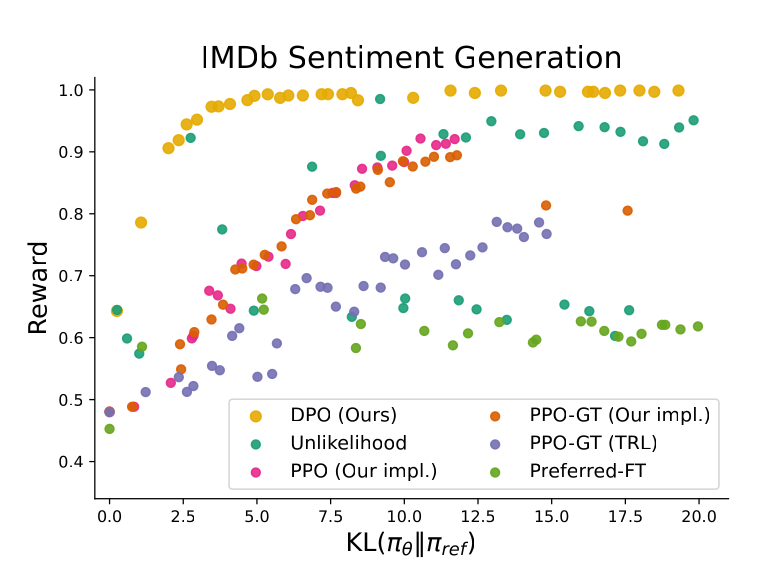
\includegraphics[width=0.7\textwidth]{images/sentiment_result.png}
    \caption{exp 1}
    \end{figure}
\end{frame}

\begin{frame}{Control setting - My try }
    \begin{itemize}
        \item Dataset: IMDB, $\sim$ 20k reviews
        \item True score function is given by a sentiment classifier (a pretrained large network)
        \item $\pi_{\text{ref}}$: Fine-tuning \texttt{gpt2-large} (1.4B params) on unlabeled IMDB
        \item For \texttt{PPO}, we provide the true score function.
        \item For \texttt{DPO}, given a prompt, we sample 4 responses for each prompt, and create 6 preference pairs.
        % \item Training take about 1h properly due to very short sentences.
    \end{itemize}
    \begin{table}
        \centering
        \caption{About an hour training for each method}
        \begin{tabular}{|c|c|c|c|}
            \hline
            & $\pi_{\text{ref}}$  & $\pi_{\texttt{ppo}}$ & $\pi_{\texttt{dpo}}$  \\ \hline
            Sentiment score & 0.625 & 0.86 & 0.99 \\\hline
            KL & 0. & 1.7 & {\red -26.6} \\\hline
        \end{tabular}
    \end{table}
\end{frame}

\begin{frame}{Result on other tasks}
    
\end{frame}

\begin{frame}{Extensions}
    \begin{itemize}
        \item Assuming preference pairs are noisy due to annotator's imperfection, 
            \begin{align*}
            &z  \sim  \text{Bern}(\sigma(r(\bm{x}, \bm{y}_1) - r(\bm{x}, \bm{y}_2))) \\
            &\ell \sim \textsf{Pr}(\ell ' \mid z)
            \end{align*}
        \item In \citep{christiano2017deep}, some pairs annotations are just uniformed selected $\Rightarrow$ outliers.
        \item Instead of pairwise preferences, we can consider a best-choice preferences: Given a prompt $\bm{x}$ and $L$ responses, the label is the best response. \citep{ziegler2019fine}.
        \item Assuming existence of score function might not hold in general
        \item What about $\Dkl{\pi_{\text{ref}}}{\pi_{\boldsymbol \theta}}$
    \end{itemize}
\end{frame}


% \begin{frame}
%     Pros
%     \begin{itemize}
%         \item Avoid the 2-step procedure
%         \item Much simpler optimization problem
%     \end{itemize}
%     Cons
%     \begin{itemize}
%         \item What if $r$ is given, such as a control sentiment problems.
%     \end{itemize}
%     What are the other preference models?
%     \begin{itemize}
%         \item Asking for the best response among $l$ responses \citep{ziegler2019fine}
%         \item \citep{christiano2017deep} incorporates ``outlier'' samples
%     \end{itemize}
% \end{frame}


% \begin{frame}{Some heuristic, technical details}
%     \begin{itemize}
%         \item KL should be within 10.
%     \end{itemize}
% \end{frame}
%
% \begin{frame}
%     \[
%     P(\bm{x}) = 
%     P(x_n \mid x_{n-1}, x_{n-2}, \ldots , x_1)
%     P(x_{n-1} \mid x_{n-2}, x_{n-3}, \ldots , x_1)
%     \ldots 
%     P(x_2 \mid x_1)
%     \] 
% \end{frame}

% \begin{frame}{Questions}
%     \begin{itemize}
%         \item What if we use DKL between $\pi_{\text{ref}}$ and $\pi_{\boldsymbol \theta}$?
%         \item What's secrete they talking about?
%     \end{itemize}
%     \[
%     \Dkl{P}{Q} = \mathop{\mathbb{E}}_{x \sim P} \left[ \log P(x) - \log Q(x) \right]
%     \] 
% \end{frame}

% \begin{frame}{Thoughts}
%     The second term
%     \begin{align*}
%     \mathop{\mathbb{E}}_{\bm{x} \sim \mathcal{D}} \left[  \Dkl{\pi_{\boldsymbol \theta}(\bm{y} \mid \bm{x})}{\pi^{\text{ref}}(\bm{y} \mid \bm{x})}\right]
%     &= \mathop{\mathbb{E}}_{\bm{x} \sim \mathcal{D}, \bm{y} \sim \pi_{\boldsymbol \theta}(\cdot \mid \bm{x})} \left[ \log \pi_{\boldsymbol \theta}(\bm{y} \mid \bm{x}) - \log \pi^{\text{ref}}(\bm{y} \mid \bm{x}) \right] \\
%     &\approx \dfrac{1}{n} \sum^{n}_{i=1} \mathop{\mathbb{E}}_{\bm{y} \sim \pi_{\boldsymbol \theta}(\cdot \mid \bm{x}_i)} \left[ \log \pi_{\boldsymbol \theta}(\bm{y} \mid \bm{x}_i) - \log \pi^{\text{ref}}(\bm{y} \mid \bm{x}_i) \right],
%     \end{align*} 
%     which is still ``hard'' to optimize.
%     What about 
%     \begin{align*}
%     \mathop{\mathbb{E}}_{\bm{x} \sim \mathcal{D}} \left[  \Dkl{\pi^{\text{ref}}(\bm{y} \mid \bm{x})}{\pi_{\boldsymbol \theta}(\bm{y} \mid \bm{x})}\right]
%     &= \mathop{\mathbb{E}}_{\bm{x} \sim \mathcal{D}, \bm{y} \sim \pi^{\text{ref}}(\cdot \mid \bm{x})} \left[ \log \pi^{\text{ref}}(\bm{y} \mid \bm{x}) - \log \pi_{\boldsymbol \theta}(\bm{y} \mid \bm{x})   \right] \\
%     &\approx \dfrac{1}{nm} \sum^{n}_{i=1} \sum^{m}_{j=1} \left[\log \pi^{\text{ref}}(\bm{y}_{ij} \mid \bm{x}_i) - \log \pi_{\boldsymbol \theta}(\bm{y}_{ij} \mid \bm{x}_i)  \right],
%     \end{align*} 
%     where we sample $m$ responses $\bm{y}_{i1}, \ldots , y_{im}$ from $\pi^{\text{ref}}(\cdot \mid \bm{x})$ for each prompt $\bm{x}_i$.
% \end{frame}
%
% \begin{frame}{Thoughts}
%     For the first term, assuming $r_{\boldsymbol \phi^{\natural}}(\bm{x}, \bm{y})$ is known,
%     \[
% \mathop{\mathbb{E}}_{\bm{x} \sim \mathcal{D}, { \bm{y} \sim \pi_{\boldsymbol \theta}(\cdot \mid \bm{x})}} \left[  { r_{\boldsymbol \phi^{\natural}}(\bm{x}, \bm{y})} \right]
% \approx \dfrac{1}{n} \sum^{n}_{i=1} \mathop{\mathbb{E}}_{\bm{y} \sim \pi_{\boldsymbol \theta}(\cdot \mid \bm{x})} r_{\boldsymbol \phi^{\natural}}(\bm{x}_i, \bm{y}).
%     \] 
%     \begin{itemize}
%         \item Is this the same issue as in policy gradient? Yes, and it is still feasible to get an estimate of the gradient. However,
%         \item How PPO solves it? How RL solves it? It is quite similar to TRPO.
%         \item And how about VAE trick?
%     \end{itemize}
% \end{frame}


\begin{frame}{Preference Optimization with the Pairwise Cringe Loss}
    \fullcite{xu2023some}
    Alignment samples can be in different forms:
    \begin{itemize}
        \item Supervised setting: ($\bm{x}, \bm{y}$ )
        \item Binary feedback: ($\bm{x}^{+}, \bm{y}^{+}, \bm{x}^{-}, \bm{y}^{-}$ )
        \item Binary preference: ($\bm{x}, \bm{y}_1, \bm{y}_2$ )
    \end{itemize}
\end{frame}

\begin{frame}
    Cringe loss is originally applied to Binary feedback data:
    \begin{align*}
    &\mathcal{L}_{\text{BIN}}(\bm{x}^{-}, \bm{y}^{-}, \bm{x}^{+}, \bm{y}^{+}) = \mathcal{L}_{\text{CE}} + \mathcal{L}_{\text{Cr}} \\
    &\mathcal{L}_{\text{CE}}(\bm{x}^{+}, \bm{y}^{+}) = -\log \textsf{Pr}(\bm{y}^{+} \mid \bm{x}^{+}) \\
    &\mathcal{L}_{\text{Cr}}(\bm{x}^{-}, \bm{y}^{-}) = -\log \sum_{t} \log \dfrac{\exp(s_t^{*})}{\exp(s_t^{*}) + \exp(s_t[y_t^{-}])},
    \end{align*}
    where we feed the prompt $\bm{x}^{-}$ to the model, and ask it to generate an output of length $T$:
    \begin{itemize}
        \item At the $t$-th token, we select top $k$ tokens according model's prob output $s_t^{1}, \ldots , s_t^{k}$.
        \item Normalizing probability over these tokens by applying softmax function.
        \item Sample an index $z \sim \text{Categorical}(s_t^{1}, \ldots , s_t^{k}), z \in [k]$ .
        \item $s_t^{*} = s_t^{z}$.
    \end{itemize}
\end{frame}
\begin{frame}{Apply Cringe Loss to Pairwise Preference data}
    They propose to use the following loss on pairwise preference data
    \[
    \mathcal{L}_{\text{Pair}}(\bm{x}, \bm{y}_1, \bm{y}_2) = g(\bm{x}, \bm{y}_1, \bm{y}_2) \mathcal{L}_{\text{BIN}}(\bm{x}, \bm{y}_1, \bm{x}, \bm{y}_2),
    \] 
    where 
    \begin{align*}
    &g(\bm{x}, \bm{y}_1, \bm{y}_2) = \sigma (b - M(\bm{x}, \bm{y}_1, \bm{y}_2)),\\
    &M(\bm{x}, \bm{y}_1, \bm{y}_2) = \log \textsf{Pr}(\bm{y}_1 \mid \bm{x}) - \log \textsf{Pr}(\bm{y}_2 \mid \bm{x}).
    \end{align*}
\end{frame}

\begin{frame}{Result}
\begin{figure}
\centering    
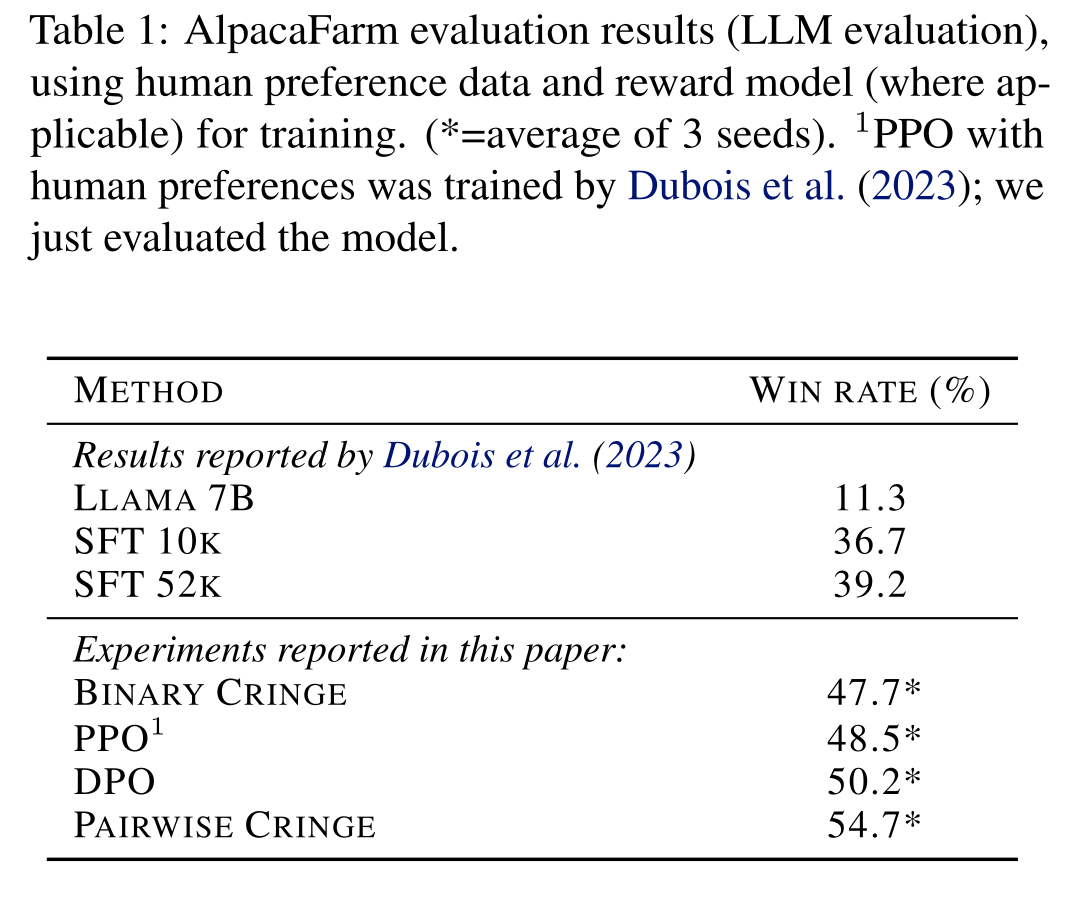
\includegraphics[width=0.5\textwidth]{images/cr_loss.png}
\caption{Image}
\end{figure}
\end{frame}


\end{document}
